\section{이론적 배경}

\subsection{Micro Touch와 모터의 조절}

그림3 이 바로 Micro Touch로, 시중에 나와 있는 모터 초점 조절 장치이다. 이를 옆의 컴퓨터와 연결하여 컴퓨터에서도 ASCOM이라는 프로그램을 이용하여 원격으로 모터의 초점을 맞출 수 있도록 설정할 
\begin{wrapfigure}{l}{0.25\textwidth}
	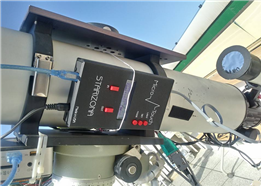
\includegraphics[width=1\linewidth]{telescope1}
	\caption{Micro Touch가 달린 천체망원경}
	\label{fig:telescope1}
\end{wrapfigure}
수가 있다. 그림3에서 나온 위의 두 버튼(IN, OUT)은 각각 초점을 맞추기 위해 망원경의 길이를 줄이거나 늘일 수 있는 버튼이다. Micro Touch를 수동 혹은 자동으로 작동시켜 IN 또는 OUT의 명령을 내렸을 경우, 모터 초점 조절 장치가 작동하게 된다. 이 모터 초점 조절 장치는 모터를 움직여 천체망원경의 경통의 길이를 조절할 수 있도록 한다. 경통의 길이가 변화하면 그에 따라서 빛이 퍼지는 정도가 달라지므로 이를 잘 조정하면 망원경으로 관측하는 천체의 초점을 맞출 수 있다.

\subsection{온습도 감지기를 이용한 온도 및 습도의 조절}

\begin{wrapfigure}{l}{0.05\textwidth}
	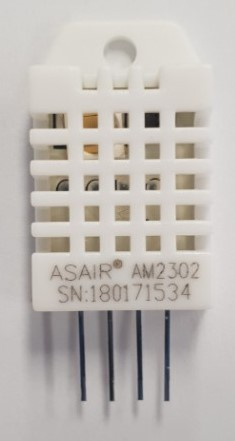
\includegraphics[width=1\linewidth]{DHT22}
	\caption{DHT22}
	\label{fig:DHT22}
\end{wrapfigure}
이 연구를 진행하는 데 Arduino를 사용하는 것이 가장 기본이라고 판단하였기 때문에 Arduino로 실행할 수 있는 것 중 쉬운 축이라고 생각되는 온습도 감지기(DHT22)를 활용하여 온습도를 측정하는 일이었다. 기판을 짜고 코드를 입력하면 Serial Monitor에 온도와 습도가 delay 함수에서 지정한 만큼의 간격을 두고 계속 출력된다. 이를 응용하여 OLED(OLED1306)에 온도와 습도를 실시간으로 출력하는 프로그램을 만들 수도 있다.

\subsection{스테핑 모터}

\subsubsection{스테핑 모터의 종류}

스테핑 모터의 종류는 크게 bipolar와 unipolar 타입으로 나눌 수 있다. 하나는 2상 6선식이라고 불리는 bipolar 스테핑 모터로, 전선이 6개가 연결되어 있다. 2상 4선식이라고도 불리는 unipolar 타입은 전선이 4개가 연결된 모터로, 구동 방식은 bipolar 타입과 크게 다르지 않다.\\
본 논문에서 사용된 스테핑 모터는 2상 6선식 모터이지만, 그 구동 방식이 비슷하므로 bipolar 스테핑 모터에서 필요 없는 2번 선과 5번 선을 제거하는 것으로 bipolar 스테핑 모터를 unipolar 스테핑 모터처럼 구동할 수 있다.

\subsubsection{스테핑 모터의 작동 원리}

\begin{wrapfigure}{l}{0.5\textwidth}
	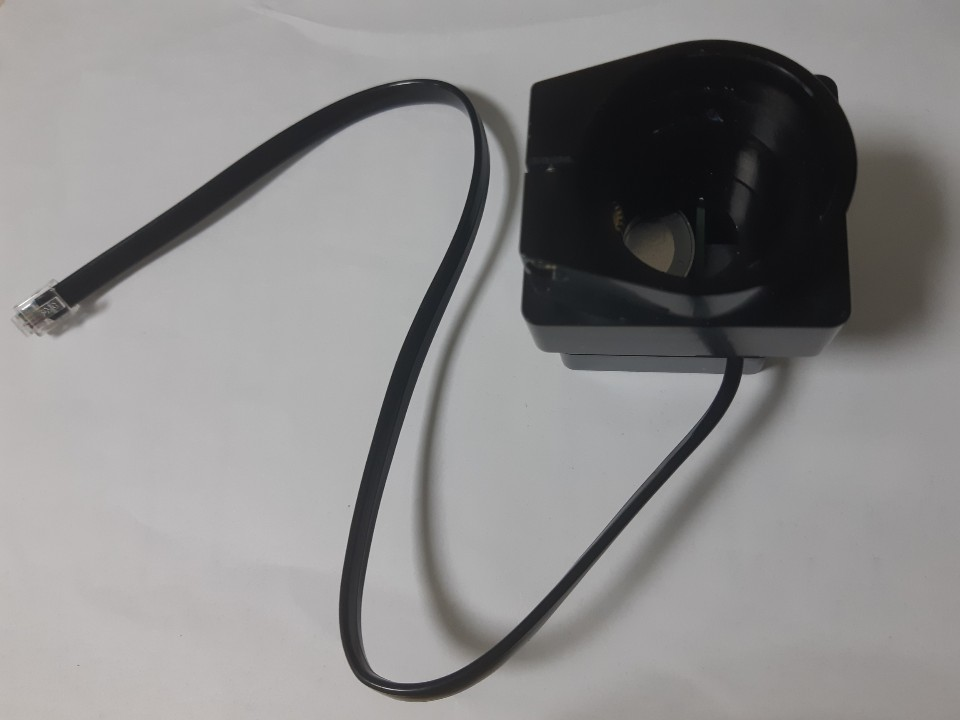
\includegraphics[width=1\linewidth]{stepmotor}
	\caption{스테핑 모터}
	\label{fig:stepmotor}
\end{wrapfigure}
우리가 실생활에서 볼 수 있는 모터 대부분은, 예를 들어 선풍기의 모터는, DC모터이다. DC모터는 전류가 흐르는 상태에서는 계속 회전하기 때문에 원하는 위치에서 멈추는 것이 어렵다. 하지만 스테핑 모터는 회전자 주위에 여러 고정자가 존재하여, 이 고정자들에 흐르는 전류의 변화량에 따라서 회전자 내부의 자석을 회전시키기 때문에, 전류의 양에 따라서 일정한 각도를 정확하게 회전시킬 수 있다. 따라서 본 연구와 같이 회전시키는 것이 중심이 아닌, 정확하게 얼마나 돌아갔는지(어느 각도만큼 돌아갔는지가 중요하게 작용할 때) 대부분 스테핑 모터를 활용하고는 한다. 이렇듯 선별로 흐르는 전류의 양에 의해 회전하는 정도와 속도를 결정할 수 있기에 흔히 ‘마이크로 스테핑’을 이용하여 전류를 여러 단계로 나누어 흘려보내어 더 정밀하게 모터를 제어하는 방법들도 존재한다. 대부분의 스테핑 모터는 1 스텝당(full step) 1.8도를 돈다고 알려져 있다.

\subsection{각 부품의 설명}

\subsubsection{Arduino Arduino NANO}

모터 초점 조절 장치 컨트롤러를 만드는 데 있어 가장 중요한 부품으로, 일종의 작은 컴퓨터와 같은 역할을 한다. Arduino는 마이크로 컨트롤러를 달고 있는 기판으로, Arduino의 여러 가지 핀에 전선을 연결한 뒤에 코딩하여 Arduino에 올리면 Arduino가 코딩된 내용을 그대로 실행할 수 있도록 하는 hardware이다. 내부에 컴퓨터 역할을 하는 MPU인 ATmega328가 탑재되어 있으며, 5V를 공급할 시에 작동한다. 크기는 45mm x 18mm이다.

\subsubsection{0.96" oled screen I2C}

Arduino와 I2C 방법으로 통신을 할 수 있는 OLED 스크린이다. 여러 가지 정보가 전달되며, 모터를 얼마나 돌릴 것인지, 혹은 얼마나 돌려져 있는지 등이 표현될 수 있다.

\subsubsection{DHT22}

온도와 습도를 측정할 수 있는 감지기로, -40~80℃의 넓은 온도 측정범위와 약 0.5℃밖에 없는 오차를 가지고 있다. 이를 통해 온도나, 렌즈의 온도 상태를 볼 수 있으며, 이를 사용하면 좀 더 정밀한 측정이 가능할 것이다.

\subsubsection{Apem MJTP1230B 버튼스위치}

누르는 버튼의 일종으로, 다리가 4개 달린 상태에서 같은 방향에 있는 2개의 전선이 연결된 방식의 버튼이다. 내부의 pull-up 저항을 활용하면 Arduino와 직접 연결하는 것으로 작동시킬 수 있다.

\subsubsection{BP5277-90}

모터를 돌리기 위해서는 12V의 전압이 필요하다. 즉, 12V의 전압을 이용하여 모터를 돌리면서 Arduino를 실행시키기 위해서는 12V를 Arduino의 입력전압인 5V까지 낮출 필요가 있다. 이에 regulator와 축전기를 활용하여 가장 안전하게 5V까지 전압을 낮출 수 있는 regulator를 선택하였다.

\subsubsection{HC-06 bluetooth}

무선통신 장치이다. 여러 가지 무선통신 장치 중에서 블루투스 module의 역할을 하고 있다.

\subsubsection{LED 3mm 90', Ohmite OD473JE}

전원이 여러 개가 존재할 수 있으므로, 모터가 돌아갈 수 있는 전압인 12V의 외부전압이 들어왔을 때만 LED가 깜빡일 수 있게 하여 모터가 돌아갈 수 있는 전압이 되었는지 확인할 수 있도록 하는 역할을 하고 있다.

\subsubsection{Panasonic EEA-GA1C100H}

모터를 돌리는 상황에서 큰 전류를 사용하기 때문에 전류가 역방향으로 흐르는 등의 문제를 방지하기 위하여 100μF의 축전기를 사용하였다.

\subsubsection{SparkFun WRL-13678 (ESP8266, ESP01)}

무선통신 장치이다. 여러 가지 무선통신 장치 중에서 WIFI 모듈을 담당한다. 입력전압이 5V가 아닌 3.3V이다.

\subsubsection{Sprague 1C10X7R104K050B}

부품별로 각각 연결된 축전기로, 모두 같은 전압 차를 가지고 있지만, 전류의 noise filtering을 하는 역할로, 필수적으로 사용되었다.

\subsubsection{TMC2100 (DRV8825)}

스테핑 모터를 돌리는 데 있어서 전류를 쉽게 조절할 수 있게 해주는 module이다. 이뿐만이 아니라 모터를 좀 더 세밀하게 돌릴 수 있게 해주는(스텝 당 돌아가는 각도를 줄여주는) 마이크로 스텝을 구현 가능한데, DRV8825의 핀 중 M1, M2, M3의 up, down을 조절하여 full step을 원래 각도와 비교하면 얼마나 적게 돌릴 것인지 결정할 수 있게 한다. 본 모델은 최대 1/32까지의 마이크로 스텝이 가능하다.

\subsubsection{TE Connectivity/AMP 5525258-3 및 Wurth Elektronik 694106301002}

12V 외부전원과 모터를 연결하는 선을 연결할 수 있게 하는 module이다.

\subsection{사용한 망원경}

\begin{wrapfigure}{l}{0.14\textwidth}
	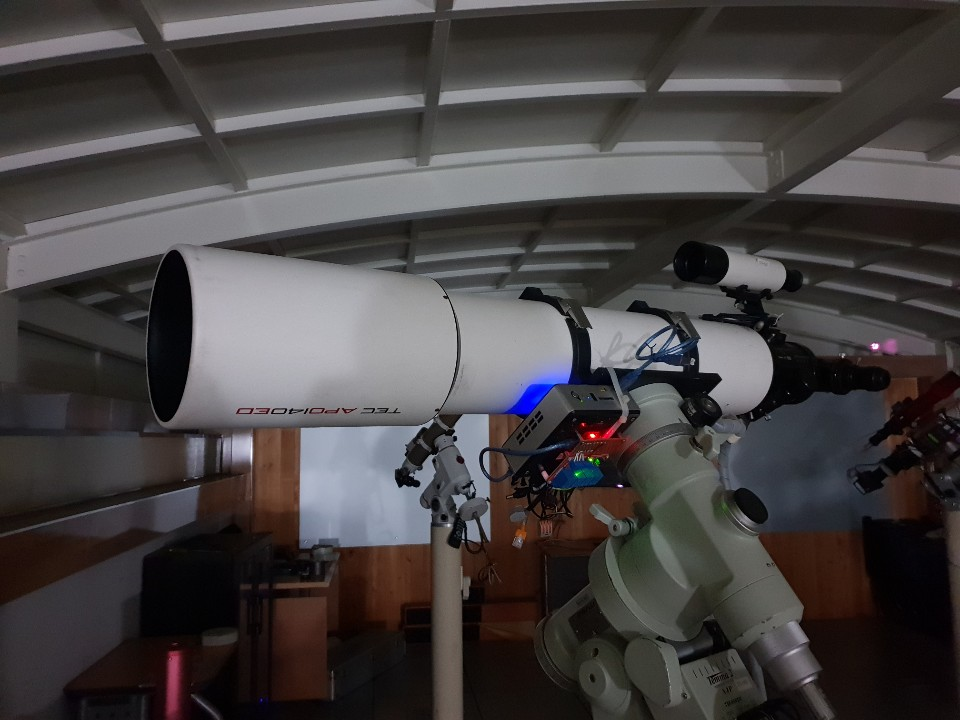
\includegraphics[width=1\linewidth]{telescope}
	\caption{사용한 망원경}
	\label{fig:telescope}
\end{wrapfigure}
TEC140 광학계에는 Starlight Instruments에서 제작한 3.5" Feather Touch Focuser가 장착되어 있다. Starlight Instruments에서는 3.5" Feather Touch Focuser에 장착할 수 있는 STEPPER MOTOR와 MICRO TOUCH FOCUSING SYSTEM을 제작하여 판매하고 있으며, 이 외에도 다른 망원경의 모터 초점 조절 장치에도 사용할 수 있도록 컨트롤러를 구현하는 것을 목표로 삼는다.

\subsection{자동초점조절 알고리즘 및 관련 논문 고찰}

이덕규 외(2014)는 복합재 광구조체와 결합하여 전자광학카메라의 영상 품질을 향상시킬 수 있는 초점 조절 장치를 개발하였다.\cite{leedukgu2014}\\
윤종환 외(2011)는 선명도에 관한 기울기를 이용하여 초점이 맞았는지를 확인하는 방법을 사용하였다.\cite{yunjonghwan2011lcd}\\
박석휘 외(2009)는 모바일 폰용 자동 초점 조절 알고리즘을 초점 값 계산 알고리즘을 이용하여 구현하였다.\cite{parksukhui2009Median}\\
이성희 외(1998)는 각 화소들의 미디언 값의 차이를 이용하여 초점을 맞추는 알고리즘을 구현하였다.\cite{leeseonghee1998Median}
